\label{sec:data}
% Main characteristics of the data set: source, type of data
% Description of variables used for the	analysis and correspondence with the (ideal) magnitudes in the empirical specification
% Descriptive statistics of the	main variables in the analysis
Data for the analysis comes from a variety of sources.
In general, we have three types of data:
\begin{itemize}
    \item Airports. Data on airports. In the network setting, these correspond to nodes in the network.
    \item Flights/connections. These datasets contain information on flights or connections between airports. As will be described in detail below, we have access to a rich dataset on US flights, and a somewhat less extensive dataset on global connections. In the network setting, this information corresponds to links in the network.
    \item Prices. Prices are generally harder to obtain in ready-to-use datasets. For this reason, we choose to scrape web-data on prices from \textit{Skyscanner}.
\end{itemize}

\subsection{Airport Data}
Data on airports comes from OpenFlights.\footnote{Available at: \url{https://openflights.org/data.html}} The dataset contains airport IATA code, name, city, country, geographical location (crs: WTS84), as well as a unique OpenFlights identifier, ICAO code and altitude. The dataset contains information on a total of 7698 airports worldwide, of which 1518 are located in the United States. Throughout the analysis, we focus on the airports that are found at least once in our dataset on flights, which is a total of 358 airports in 2018.
%Data on airports comes from two overlapping sources. Firstly, we have a dataset from the 2009 Statistical Computing Data Expo\footnote{Available at \url{http://stat-computing.org/dataexpo/2009/}}. This dataset contains information 3376 US airports, and the unique IATA\footnote{International Air Transport Association} code, airport name, city, country and geographical location in WTS84 coordinates. This dataset contains 3.376 observations of individual airports. As will be described in \ref{subsec:Flight_Data}, we only have information on flights/connections to and from a subset of these. A likely explanation is, that a number of these airports are not used for commercial air transport, but rather for e.g. training/sports purposes.\par
% Tjek at det reelt er WTS84 koordinater - det ser sådan ud.
%Secondly, we have a dataset on airports from OpenFlights\footnote{Available at: \url{https://openflights.org/data.html}}. This dataset contains the same information as the above, but further includes inter alia a unique 'OpenFlights identifier', ICAO code, and altitude. Furthermore, this dataset contains airports from all over the world.

%We will primarily use the OpenFlights data, whenever the analysis has a global scope. This dataset contains information on 7543 individual airports.

\subsection{Flights Data}
\label{subsec:Flight_Data}
Flight data comes from the Bureau of Transportation Statistics\footnote{See \url{https://openflights.org/data.html}}. We have flight data for 2007 and 2018. Each of the two datasets include information on more than 7 million commercial flights within the US. For each flight, we have a range of information, including the aircraft carrier, origin and destination (IATA coded), distance travelled, time in air date etc. Flight data can be merged with airport data using the IATA codes on airports. \medskip\\
We only use the 2007 data to assess how the network has changed from 2007 to 2018. 

%% Update: Flights data fra bts.gov og fra stat-comp (men det er igen fra bts.gov).
% Airports data: Bruger kun OpenFlights datasættet. 


%Data on airports and connections is available at: \href{https://openflights.org/data.html}{openflights.org/data.html}. See Figure \ref{fig:airports} below. The dataset includes an airport identifier (IATA code), location data (latitude and longitude), and various characteristics of the airport (country, city, altitude etc.).
%Furthermore, the dataset contains connections between airports (67,663 routes between 3,321 airports on 548 airlines). %Airports are identified using the IATA code.%we already mentioned this above
%\medskip\\
%Data on prices are scraped from the internet. Various sites contain flight prices (Skyscanner, Momondo, Flightfinder, Expedia mv.). Our choice of site will be guided by practical concerns.
%\par
%Alternative data:  \url{http://stat-computing.org/dataexpo/2009/}
%\begin{figure}[H]
%  \centering
%  \caption{Airports}
%    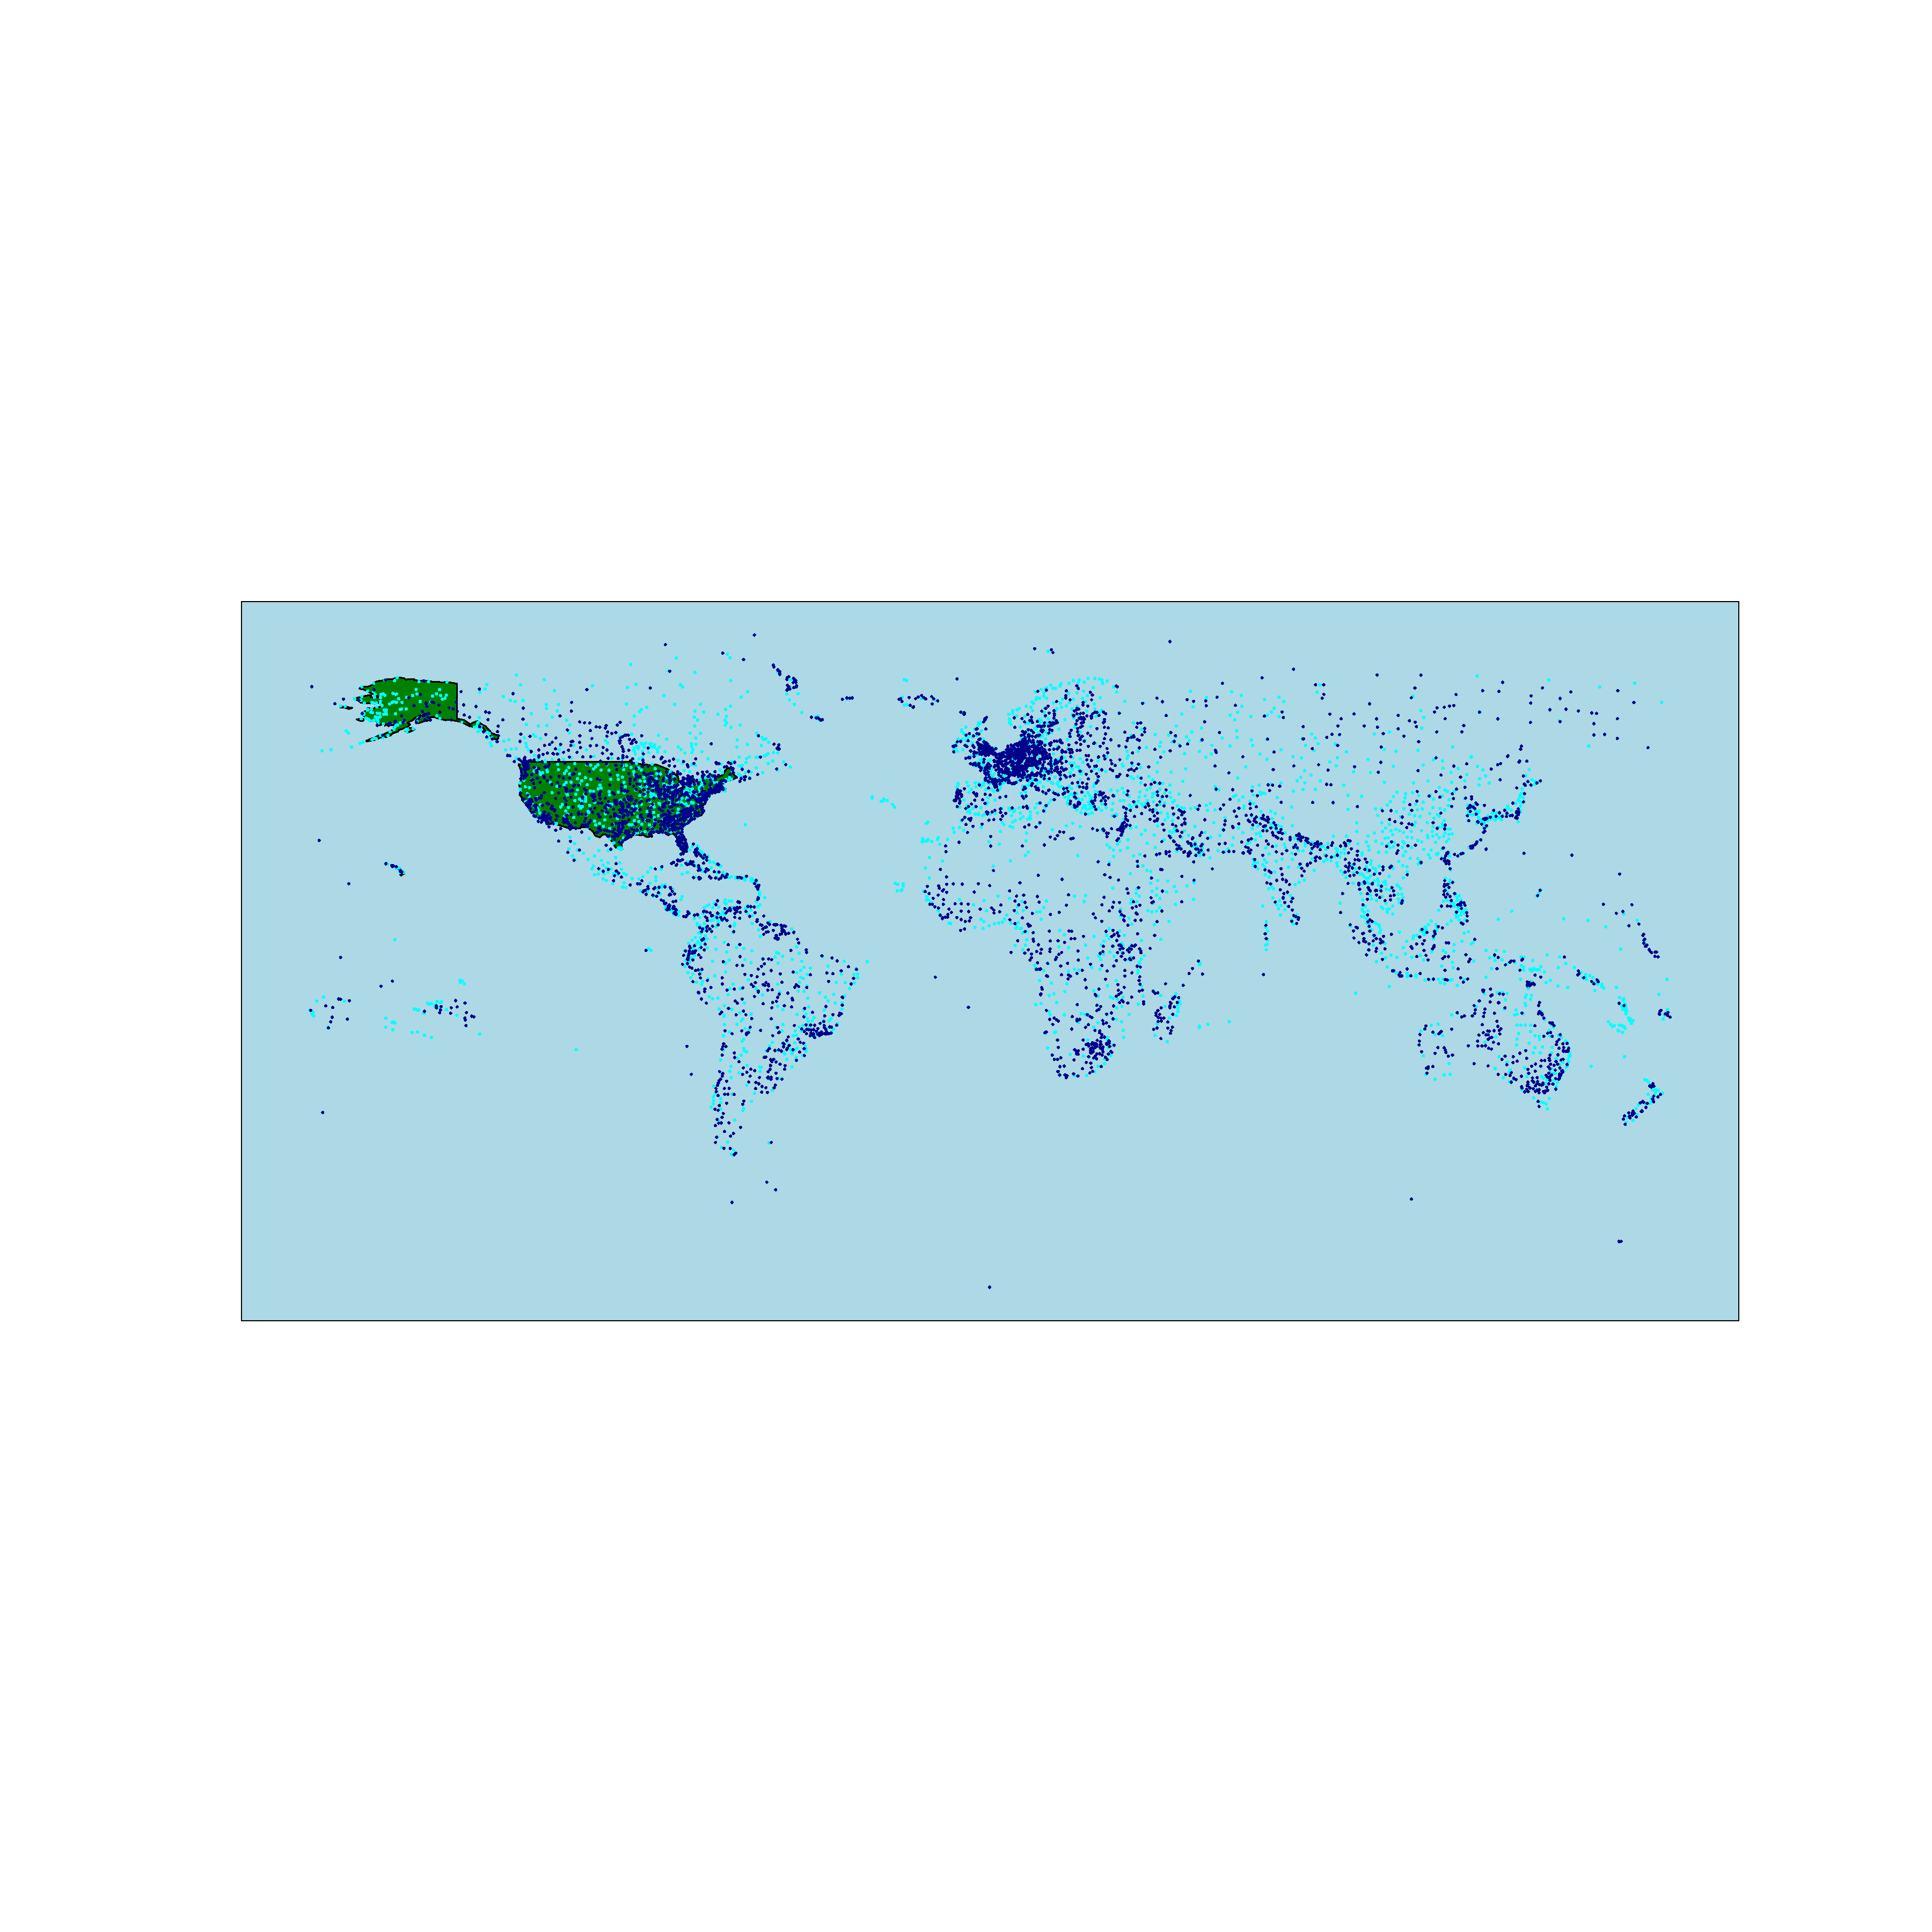
\includegraphics[width=1. \textwidth]{Exam/Airports_WorldMap}
%  \label{fig:airports}
%\end{figure}

\subsection{Price Data}
Price data are scraped from \url{skyscanner.com} using Selenium in Python. Ideally we would have preferred historical prices matching the time horizon of Flight dataset, however we have not be able to find such data. Instead we are scraping prices for all the connections. Due to limited time we have chosen to scrape prices for one specific date. This is problematic since prices shows systematic changes across weekdays, and seasonality across the year. Furthermore, our connection data includes all flight within a year and some routes might not be operated at this particular date.
The scraper function launches a browser and opens the url for a given flight at our chosen date which is May 27th. If possible the price of the cheapest direct flight is chosen. The prices of flights operated by Southwest Airlines are not shown at Skyscanner. If their flight is only one operating, the price of the cheapest indirect flight is chosen. The cheapest indirect flight is also chosen if no carrier is operating at the date.


